\documentclass[letterpaper, 12pt]{article}
\usepackage[letterpaper, top=2.5cm, bottom=2.5cm, left=3cm, right=3cm]{geometry} %margenes
\usepackage[utf8]{inputenc} %manejo de caracteres especiales
\usepackage[spanish]{babel} %manejo de encabezados de inglés a español
\usepackage{fancyhdr} %formato de los encabezados de página
\usepackage{ragged2e} %alineado real justficado
\usepackage{graphicx} %manejo de imagenes
\usepackage{amsmath} %manejo de notación matemática
\usepackage{mathtools} %manejo de notación matemática
\usepackage{blindtext} %texto de relleno
\usepackage{cancel} %permite la simbolización de cancelación de terminos
\usepackage{enumitem}[shortlabels] %listas con letras
\usepackage{amssymb} %manejo de simbolog►1a matematica

\pagestyle{fancy}
\fancyhf{}
\rfoot{\thepage}

\begin{document}
\setcounter{page}{1}
\thispagestyle{fancy}
\lhead{\textbf{Tarea 5, U2}}
\rhead{\textbf{21/10/2020}}
\section*{Curvas planas, ecuaciones paramétricas y coordenadas polares}
\subsection*{Grafíca los puntos de la tangente horizontal y vertical de la sig. ecuación, y a la misma ecuación: }
\[r=3-3\sin\theta,\, \theta\tan_{\text{horizontal}}=\frac{\pi}{6},\frac{3\pi}{2}, \frac{5\pi}{6};\,\theta\tan_{\text{vertical}}=\frac{7\pi}{6},\frac{11\pi}{6};\]
\subsubsection*{Calculos: }
Para \(\tan_{\text{horizontal}}\):
\[\begin{matrix}
    \theta&\frac{\pi}{6}&\frac{3\pi}{2}&\frac{5\pi}{6}\\
    r&1.5&6&1.5
\end{matrix}\]
Para \(\tan_{\text{vertical}}\):
\[\begin{matrix}
    \theta&\frac{7\pi}{6}&\frac{11\pi}{6}\\
    r&4.5&4.5
\end{matrix}\]
\subsubsection*{Gráficas:}
\begin{center}
    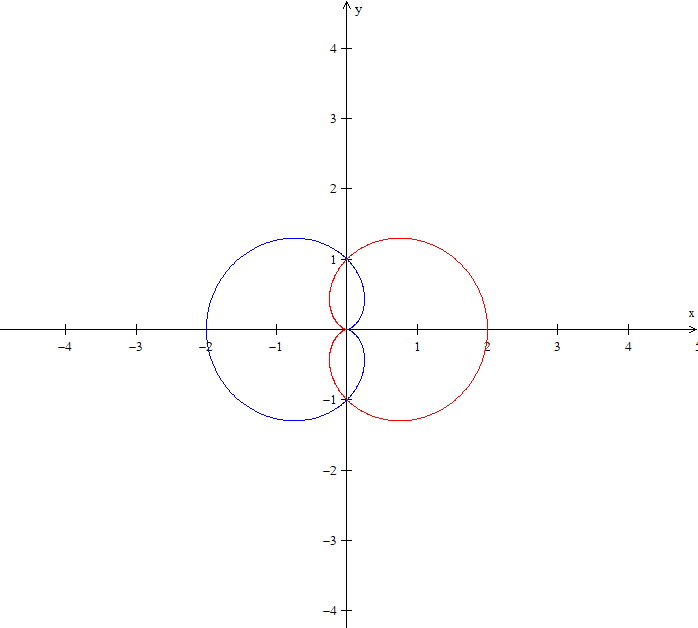
\includegraphics{Capture.png}
\end{center}
\end{document}